\begin{figure*}[t]
\centering
\subfloat[Linear Heads by Generator\label{tab:cross_model_results}]{\parbox[t][2.9cm][t]{0.24\textwidth}{\centering\vspace*{0.3cm}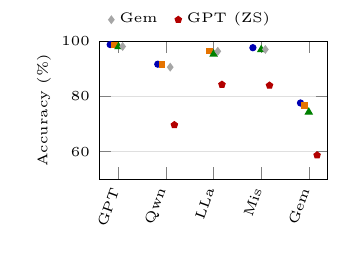
\begin{tikzpicture}\begin{axis}[ymajorgrids, grid style={gray!25}, tick label style={font=\tiny}, label style={font=\tiny}, title style={font=\tiny}, legend style={font=\tiny, draw=none, fill=none, at={(0.5,1.02)}, anchor=south}, legend columns=3, scale only axis, width=2.9cm, height=1.75cm, legend style={overlay}, ylabel shift=-3pt, symbolic x coords={GPT,Qwn,LLa,Mis,Gem}, xtick={GPT,Qwn,LLa,Mis,Gem}, x tick label style={rotate=70,anchor=east}, ylabel={Accuracy (\%)}, ymin=50, ymax=100]\addplot[only marks,mark=*,mark size=1.1pt,color=blue!70!black,xshift=-3.0pt] coordinates {(GPT,98.83)(Qwn,91.71)(Mis,97.70)(Gem,77.64)};\addplot[only marks,mark=square*,mark size=1.0pt,color=orange!90!black,xshift=-1.5pt] coordinates {(GPT,98.67)(Qwn,91.61)(LLa,96.51)(Gem,76.80)};\addplot[only marks,mark=triangle*,mark size=1.4pt,color=green!50!black] coordinates {(GPT,98.07)(LLa,95.40)(Mis,96.99)(Gem,74.33)};\addplot[only marks,mark=diamond*,mark size=1.3pt,color=gray!70,xshift=1.5pt] coordinates {(GPT,98.14)(Qwn,90.64)(LLa,96.40)(Mis,97.07)};\addplot[only marks,mark=pentagon*,mark size=1.2pt,color=red!70!black,xshift=3.0pt] coordinates {(Qwn,69.67)(LLa,84.33)(Mis,84.00)(Gem,58.67)};\legend{LLa,Mis,Qwn,Gem,GPT (ZS)}\end{axis}\end{tikzpicture}}}\hfill
\subfloat[Zero-Shot by Generator\label{tab:zero_shot_all}]{\parbox[t][2.9cm][t]{0.24\textwidth}{\centering\vspace*{0.3cm}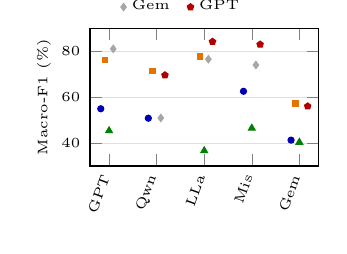
\begin{tikzpicture}\begin{axis}[ymajorgrids, grid style={gray!25}, tick label style={font=\tiny}, label style={font=\tiny}, title style={font=\tiny}, legend style={font=\tiny, draw=none, fill=none, at={(0.5,1.02)}, anchor=south}, legend columns=3, scale only axis, width=2.9cm, height=1.75cm, legend style={overlay}, ylabel shift=-3pt, symbolic x coords={GPT,Qwn,LLa,Mis,Gem}, xtick={GPT,Qwn,LLa,Mis,Gem}, x tick label style={rotate=70,anchor=east}, ylabel={Macro-F1 (\%)}, ymin=30, ymax=90]\addplot[only marks,mark=*,mark size=1.1pt,color=blue!70!black,xshift=-3.0pt] coordinates {(GPT,54.93)(Qwn,50.82)(Mis,62.54)(Gem,41.28)};\addplot[only marks,mark=square*,mark size=1.0pt,color=orange!90!black,xshift=-1.5pt] coordinates {(GPT,76.21)(Qwn,71.39)(LLa,77.57)(Gem,57.35)};\addplot[only marks,mark=triangle*,mark size=1.4pt,color=green!50!black] coordinates {(GPT,45.36)(LLa,36.65)(Mis,46.45)(Gem,40.33)};\addplot[only marks,mark=diamond*,mark size=1.3pt,color=gray!70,xshift=1.5pt] coordinates {(GPT,81.02)(Qwn,50.92)(LLa,76.52)(Mis,73.99)};\addplot[only marks,mark=pentagon*,mark size=1.2pt,color=red!70!black,xshift=3.0pt] coordinates {(Qwn,69.56)(LLa,84.15)(Mis,82.94)(Gem,56.03)};\legend{LLa,Mis,Qwn,Gem,GPT}\end{axis}\end{tikzpicture}}}\hfill
\subfloat[Zero-Shot vs.\ Linear Head\label{tab:zs_vs_ft}]{\parbox[t][2.9cm][t]{0.24\textwidth}{\centering\vspace*{0.3cm}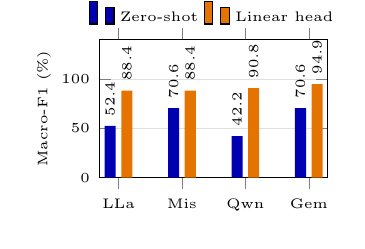
\begin{tikzpicture}\begin{axis}[ymajorgrids, grid style={gray!25}, tick label style={font=\tiny}, label style={font=\tiny}, title style={font=\tiny}, legend style={font=\tiny, draw=none, fill=none, at={(0.5,1.02)}, anchor=south}, legend columns=3, scale only axis, width=2.9cm, height=1.75cm, legend style={overlay}, ylabel shift=-3pt, ybar, bar width=4pt, symbolic x coords={LLa,Mis,Qwn,Gem}, xtick={LLa,Mis,Qwn,Gem}, ylabel={Macro-F1 (\%)}, ymin=0, ymax=140, legend columns=2, nodes near coords={\pgfmathprintnumber[fixed,zerofill,precision=1]{\pgfplotspointmeta}}, nodes near coords style={font=\fontsize{3.5}{4}\selectfont, rotate=90, anchor=west}]\addplot[fill=blue!70!black,draw=none] coordinates {(LLa,52.39)(Mis,70.63)(Qwn,42.20)(Gem,70.61)};\addplot[fill=orange!90!black,draw=none] coordinates {(LLa,88.38)(Mis,88.43)(Qwn,90.79)(Gem,94.87)};\legend{Zero-shot,Linear head}\end{axis}\end{tikzpicture}}}\hfill
\subfloat[Paired Bootstrap Tests\label{tab:significance}]{\parbox[t][2.9cm][t]{0.24\textwidth}{\centering\vspace*{0.3cm}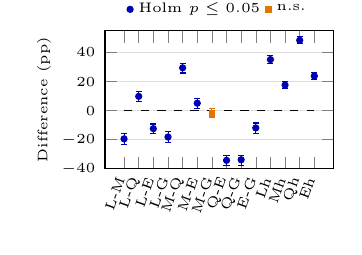
\begin{tikzpicture}\begin{axis}[ymajorgrids, grid style={gray!25}, tick label style={font=\tiny}, label style={font=\tiny}, title style={font=\tiny}, legend style={font=\tiny, draw=none, fill=none, at={(0.5,1.02)}, anchor=south}, legend columns=3, scale only axis, width=2.9cm, height=1.75cm, legend style={overlay}, ylabel shift=-3pt, symbolic x coords={L-M,L-Q,L-E,L-G,M-Q,M-E,M-G,Q-E,Q-G,E-G,Lh,Mh,Qh,Eh}, xtick={L-M,L-Q,L-E,L-G,M-Q,M-E,M-G,Q-E,Q-G,E-G,Lh,Mh,Qh,Eh}, x tick label style={rotate=70,anchor=east}, ylabel={Difference (pp)}, ymin=-40, ymax=55, legend columns=2]\addplot[only marks,mark=*,mark size=1.1pt,color=blue!70!black,error bars/.cd,y dir=both,y explicit,error bar style={line width=0.3pt}] coordinates {(L-M,-19.53)+=(0,3.48)-=(0,3.57)(L-Q,9.78)+=(0,3.26)-=(0,3.54)(L-E,-12.47)+=(0,3.21)-=(0,3.21)(L-G,-18.25)+=(0,3.87)-=(0,3.59)(M-Q,29.46)+=(0,3.26)-=(0,3.59)(M-E,5.07)+=(0,3.47)-=(0,3.66)(Q-E,-34.33)+=(0,3.61)-=(0,3.43)(Q-G,-33.92)+=(0,3.11)-=(0,3.66)(E-G,-11.98)+=(0,3.37)-=(0,3.67)(Lh,35.15)+=(0,2.59)-=(0,2.41)(Mh,17.54)+=(0,2.73)-=(0,2.48)(Qh,48.46)+=(0,2.74)-=(0,2.41)(Eh,23.81)+=(0,2.56)-=(0,2.59)};\addplot[only marks,mark=square*,mark size=1.0pt,color=orange!90!black,error bars/.cd,y dir=both,y explicit,error bar style={line width=0.3pt}] coordinates {(M-G,-1.85)+=(0,3.19)-=(0,3.13)};\addplot[dashed,black,line width=0.3pt] coordinates {(L-M,0)(Eh,0)};\legend{Holm $p\le0.05$,n.s.}\end{axis}\end{tikzpicture}}}
\caption{Cross-generator and zero-shot evaluation (GPT: GPT-4o; Qwn: Qwen3.5-2B; LLa: LLaMA-2-7B-chat; Mis: Mistral-7B-Instruct; Gem: Gemma-7B). (a)~Accuracy of linear heads on frozen backbones by test generator; GPT-4o is evaluated zero-shot (ZS) on 300 evaluation posts per generator. (b)~Zero-shot Macro-F1 on the 1{,}500-post evaluation set; a classifier is not scored on its own posts. (c)~Zero-shot vs.\ linear-head Macro-F1 for the same backbones, averaged across generators. (d)~Paired bootstrap differences with 95\% CIs (1{,}000 resamples, Holm-adjusted) between zero-shot classifiers (A-B: A minus B) and of each linear head over its zero-shot backbone (Xh); G: GPT-4o, Q: Qwen, L: LLaMA-2, M: Mistral, E: Gemma.}
\label{fig:generators}
\vspace{-0.3cm}
\end{figure*}